\documentclass[12pt]{beamer}
 
\usepackage[utf8]{inputenc} 
\usepackage[T1]{fontenc}
\usepackage{lmodern}
\usepackage{graphicx}
\usepackage{pslatex}

\definecolor{bg}{RGB}{235,235,235}
\newcommand{\class}[1]{\colorbox{bg}{\textcolor{red}{\usefont{OT1}{cmtt}{m}{n}#1}}}
 
\usetheme[nat,TPlrimage=Set,logostyle=none,headstyle=institute]{Frederiksberg}

\title{Set Multijoueurs}
\subtitle{Application Android et programmation concurrente}
\author{Zhixing CAO, Yuxiang LI}
\institute[Project INF 431]{X2013}
\date[]{\today}
 
\begin{document}

\frame[plain]{\titlepage}

\section{Introduction}
\begin{frame}
\tableofcontents[currentsection]
\end{frame}    

\begin{frame}
\frametitle{Set !}

Set! © est un jeu de cartes qui peut se jouer à un ou plusieurs joueurs. Le jeu est constitué de 81 cartes toutes différentes qui se distinguent selon 4 caractéristiques :
\begin{itemize}
\item Nombre : 1, 2 ou 3 objets
\item Couleur : rouge, vert ou bleu
\item Remplissage : vide, hachuré ou plein
\item Forme : ovale, rectangle ou losange
\end{itemize}

\begin{figure}
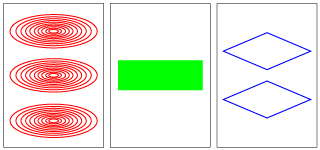
\includegraphics[height=2cm]{set1.jpg}
\end{figure}
\end{frame}

\begin{frame}
\frametitle{Règle du jeu}
\begin{itemize}
\item Score et pénalité
\item Premier arrivé, premier servi
\end{itemize}
\end{frame}

\section{Implémentation en Java}
\begin{frame}
\tableofcontents[currentsection]
\end{frame}    

\begin{frame}
\frametitle{Android}
4 classes :
\begin{itemize}
\item \class{Card}
\item \class{CardSet}
\item \class{CardView}
\item \class{MainActivity}
\end{itemize}
\end{frame}

\begin{frame}
\frametitle{Serveur}
Mode de communication :
\begin{itemize}
\item Modifier les cartes : V{\textvisiblespace}$pos_1${\textvisiblespace}$card_1${\textvisiblespace}$pos_2${\textvisiblespace}$card_2$ ...
\item Incrémenter le score : S{\textvisiblespace}$card_1${\textvisiblespace}$card_2${\textvisiblespace}$card_3$
\item (Serveur) Afficher le scoreboard : B{\textvisiblespace}$score_1${\textvisiblespace}$score_2$ ...
\item Débloquer tous les joueurs : M
\item Faire sortir le joueur : E
\item Informer sur l'état de blocage : F
\item (Client) Demander le scoreboard : B
\item (Client) Actualiser le score : N{\textvisiblespace}$score$
\item Soumettre le résultat : S{\textvisiblespace}$pos_1${\textvisiblespace}$card_1${\textvisiblespace}$pos_2${\textvisiblespace}$card_2$ ...
\item Quitter le jeu : E
\end{itemize}
\end{frame}

\begin{frame}
\frametitle{Différents threads}
Serveur :
\begin{itemize}
\item Main
\item Clients : un client, un thread
\item Détection de blocage
\item Détection de joueur muet
\end{itemize}

Client :
\begin{itemize}
\item Main (UI) 
\item Timer et Scoreboard
\item Message Socket
\item etc. : \class{DelayThread}
\end{itemize}
\end{frame}

\section{Détails techniques}
\begin{frame}
\tableofcontents[currentsection]
\end{frame}    

\begin{frame}
\frametitle{Quelques classes Java / Android}
\begin{itemize}
\item Reflect : \class{Class<T>} et  \class{Field}
\item \class{Handler}
\item \class{ExecutorService}
\item \class{Callable<T>} et \class{Future<T>}
\end{itemize}
\end{frame}

\section{Démonstration}
\begin{frame}
\tableofcontents[currentsection]
\end{frame}    

\begin{frame}
\frametitle{Démonstration}
Questions ?
\end{frame}
 
\end{document}